% !TeX root = Bericht_main.tex
\subsection{Aufgabe 14/15}
\subsubsection{Gemischte Finite Elemente}
\begin{figure}[H]
	\centering
	\captionabove{Lösungen mit gemischten FEM}
	\subfigure[des Problems 'Simple']{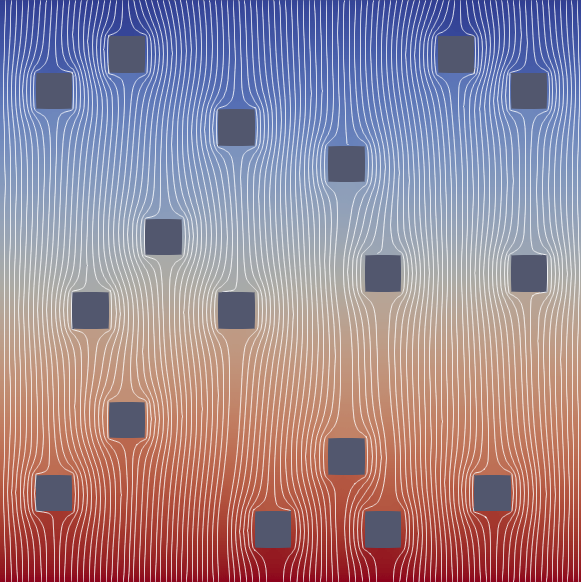
\includegraphics[width=0.49\textwidth]{../../14.1.Simple/figrand(1).png}}
	\subfigure[des Problems 'Discontinuous']{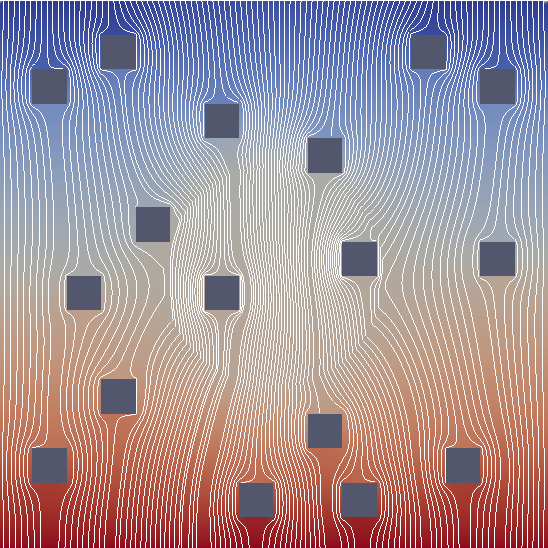
\includegraphics[width=0.49\textwidth]{../../14.1.Disc/figrand(1).png}}

\end{figure}

\begin{figure}[H]
	\centering
	\captionabove{Lösungen mit linearen FEM}
	\subfigure[des Problems 'Simple']{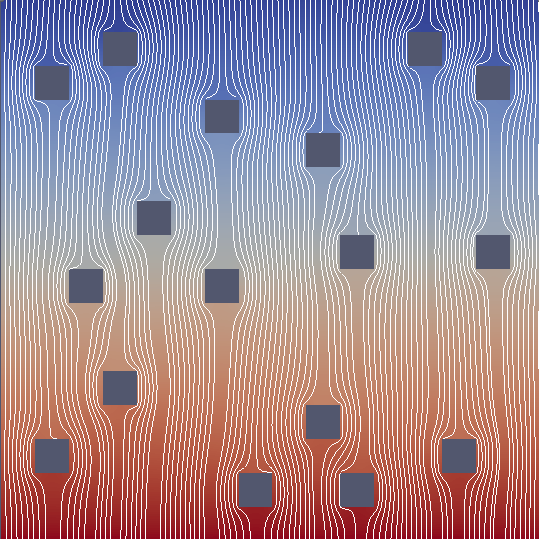
\includegraphics[width=0.49\textwidth]{../../14.1.Simple/figrandold.png}}
	\subfigure[des Problems 'Discontinuous']{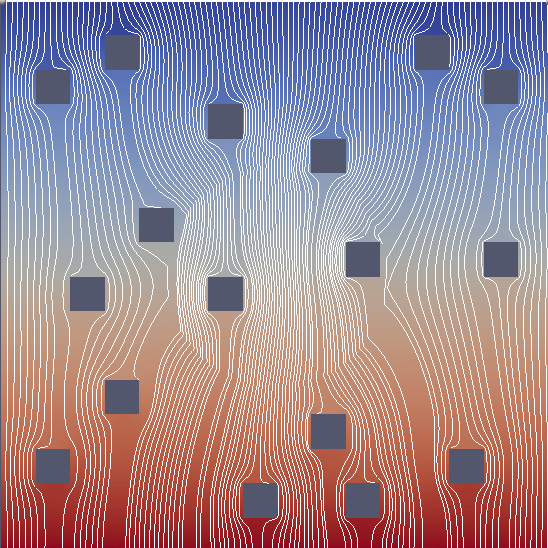
\includegraphics[width=0.49\textwidth]{../../14.1.Disc/figrandold.png}}

\end{figure}

\begin{figure}[H]
   \centering
	\captionabove{Lösung des 'LinearAffineInflowProblem'}
	{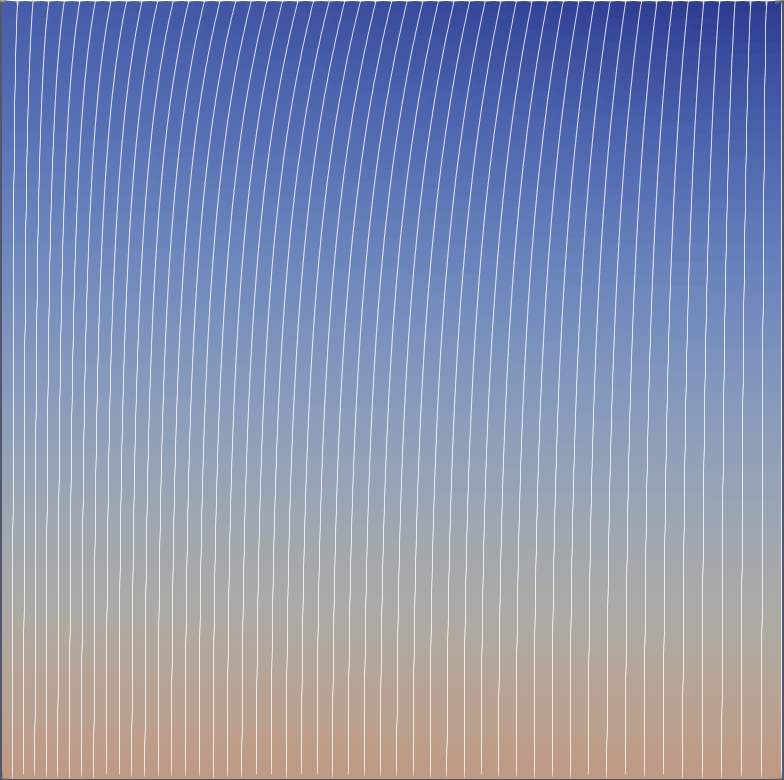
\includegraphics[width=0.49\textwidth]{../../Aufgabe14/flux.png}}
\end{figure}

Beim Lösen des in der Aufgabe gegebenen Sattelpunktproblems konnte verifiziert werden, dass bei der Verwendung von gemischten Finiten Elementen die Ein- und Ausflussbedingung für alle verwendeten Level erhalten werden.
Im Gegensatz dazu stehen die Erkenntnisse, welche wir bereits im letzten Bericht zu den linearen Finiten Elementen gewonnen haben. 
Am Deutlichsten spiegelt sich dies in der Größe 'Flux Loss' wieder, welcher bei Verwendung von gemischten Finiten Elementen unabhängig vom Level gleich 0 ist, während er unter Verwendung von linearen Finiten Elementen auf einem komplizierten Mesh nicht zu vernachlässigen ist.  \newline
In den Plots lassen sich bei genauerem Betrachten vor allem im Bereich der Steine des Meshes 'Square500' geringe Unterschiede zwischen beiden Verfahren erkennen, so 'schmiegen' sich die gemischten Finiten Elemente etwas besser an die Steine an.
Dies lässt sich bei beiden Problemen verifizieren. 


\begin{figure}[H]
	\centering
	\captionabove{gemischte Finite Elemente Methode}
		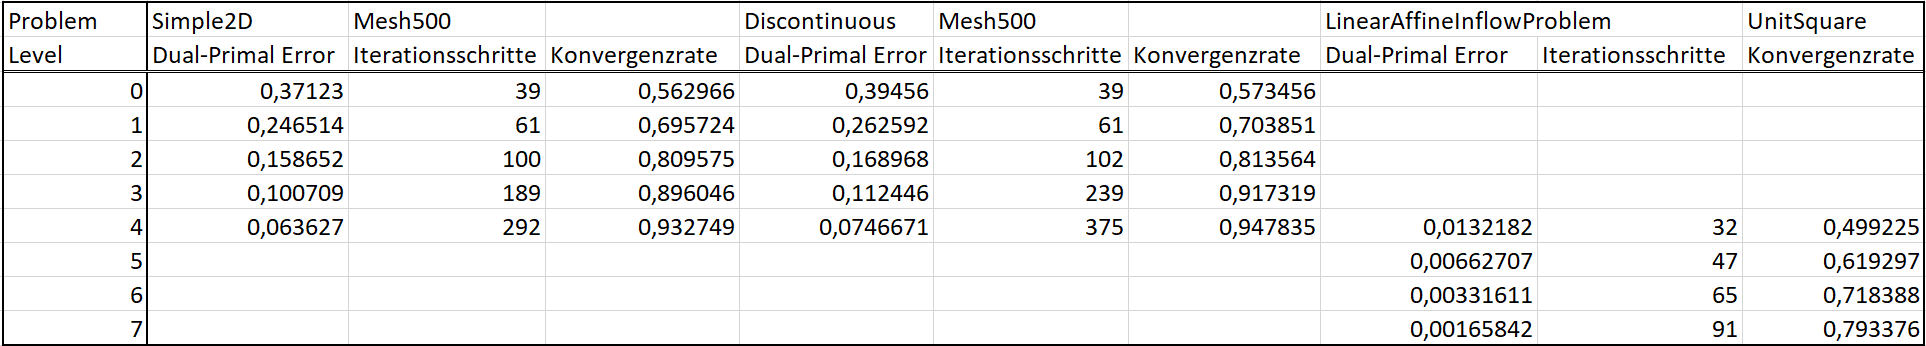
\includegraphics[width=\textwidth]{../../19/tabelle1mixed.png} 
\end{figure}

Der Fehler $e_l$ auf Level $l$ wird bei uns nun durch den Dual-Primal Error $ \left\|q_h -\kappa \nabla u_h\right\|$ berechnet. Damit lässt sich wie im vorherigen Bericht durch
\begin{align*}
  \frac{e_l}{e_{l+1}} \sim 2^p
\end{align*}
die Konvergenzrate p bestimmen. 
$\newline$
Für das Problem $Simple2D$ ergibt sich:
\begin{align*}
  \frac{e_l}{e_{l+1}} \approx 1.55 \text{ und somit } p \approx 0.636
\end{align*}
Für das Problem $Discontinuous$ ergibt sich:
\begin{align*}
  \frac{e_l}{e_{l+1}} \approx 1.52 \text{ und somit } p \approx 0.600
\end{align*}
Für das Problem \emph{LinearAffineInflowProblem} ergibt sich:
\begin{align*}
  \frac{e_l}{e_{l+1}} \approx 2.00 \text{ und somit } p \approx 1.00
\end{align*}
\subsubsection{Hybride Finite Elemente}
\begin{figure}[H]
	\centering
	\captionabove{hybride Finite Elemente Methode}
	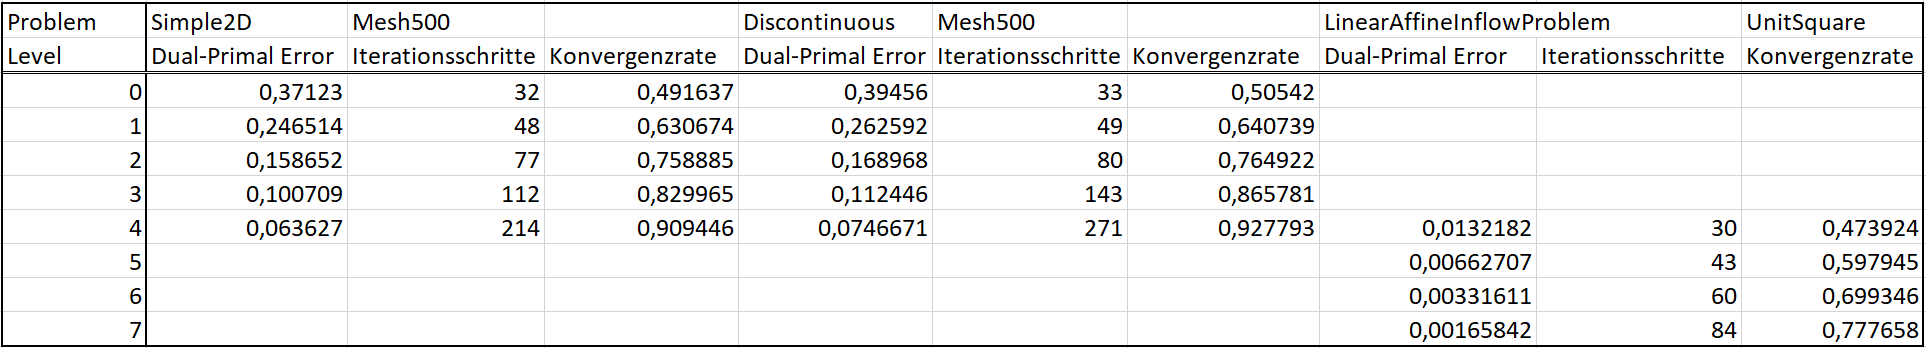
\includegraphics[width=\textwidth]{../../19/tabelle1hybrid.png} 
\end{figure}

Ein Vergleich der beiden Tabellen macht deutlich, dass bei den hybriden Finiten Elementen auf jedem Level der lineare Löser weniger Iterationsschritte bei geringerer Konvergenzrate benötigt. Weiter sieht man direkt, dass beide Finite Elemente Methoden die gleichen Ergebnisse liefern und somit auch die Level-Konvergenzrate $p$ übereinstimmt.


\subsection{Aufgabe 18/19}
\subsubsection{Vorgehen und Lösungsansätze}
\begin{figure}[H]
	\centering
	\captionabove{Problem Rock}
	\subfigure[Problemstellung]{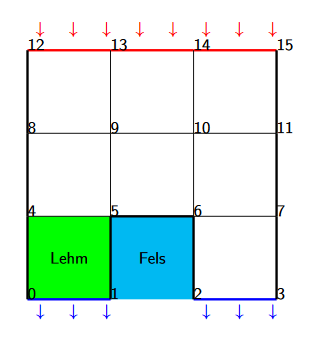
\includegraphics[width=0.4\textwidth]{../../19/problem.png}}
	\subfigure[Definitionen in Rock.geo]{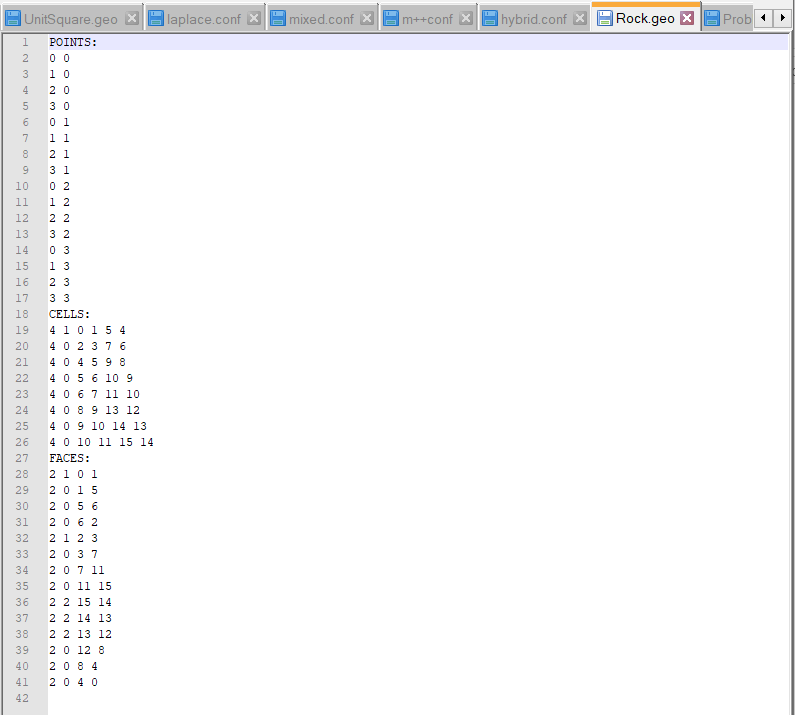
\includegraphics[width=0.59\textwidth]{../../19/rockgeo.png}}
\end{figure}
Ziel der Aufgabe war es, das in Abb.3 (a) zu sehende Problem zu implementieren bzw. vorhandene Lücken in der Implementierung zu schließen.
Zunächst haben wir dafür das Gitter samt Rändern in der Datei Rock.geo definiert. 
Auf eine nähere Erklärung des .geo-Files möchten wir an dieser Stelle verzichten und verweisen auf den ersten Praktikumsbericht.


\begin{figure}[H]
	\centering
	\captionabove{Funktion Permeability der  Klasse RockProblem}
	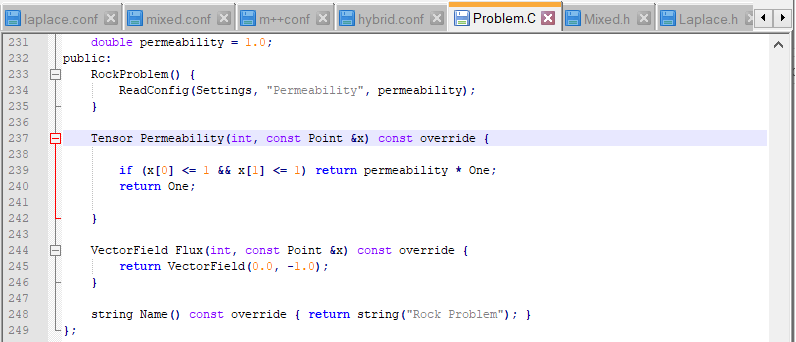
\includegraphics[width=\textwidth]{../../19/permprob.png}	
\end{figure}
In der Datei Problem.C haben wir anschließend die Funktion Permeability der Klasse RockProblem geschrieben.
Ein Punkt (x,y) ist genau dann im unteren linken Kästchen, wenn seine Maximumnorm des zugehörigen Ortsvektors kleiner oder gleich 1 ist. 
Das ist gleichbedeutend mit dem komponentenweisen Vergleich, welchen wir in Zeile 239 durchführen.


\begin{figure}[H]
	\centering
	\captionabove{Funktion OutFlowLeftRight in mixed.h}
	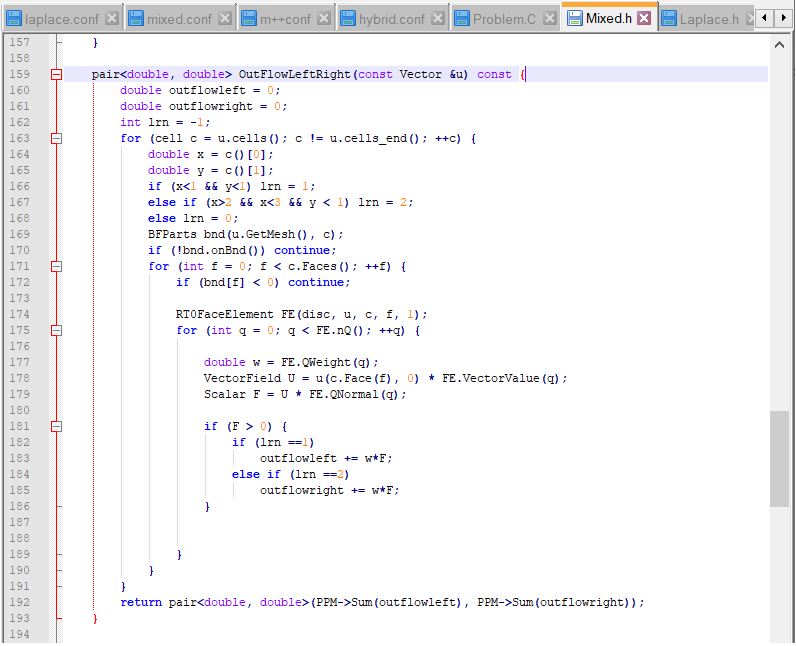
\includegraphics[width=\textwidth]{../../19/mixedoutflow.png}
	
\end{figure}
In der Funktion OutFlowLeftRight sollen dann die Ausflussmengen auf der rechten und auf der linken Seite des Steines berechnet werden. 
Dazu führen wir zunächst die temporäre Variable 'lrn' ein. Anschließend setzen wir diese auf 1, falls sich die aktuell betrachtete Zelle im Lehmblock befindet, auf 2, falls es sich um eine Zelle rechts des Steines handelt, und 0 sonst. \newline
Mit 'c()[i]' können wir dabei auf die i-te Koordinate des \underline{Zellmittelpunktes} zugreifen, man beachte dies vor allem im Zusammenhang mit den entsprechenden Abfragen. 
Nachdem wir dann wie üblich den Fluss an den äußeren Faces der entsprechenden Zelle berechnet haben, addieren wir den Ausfluss auf den entsprechenden Summationswert und geben diese Werte zuletzt zurück.

\begin{figure}[H]
	\centering
	\captionabove{Funktion OutFlowLeftRight in Laplace.h}
	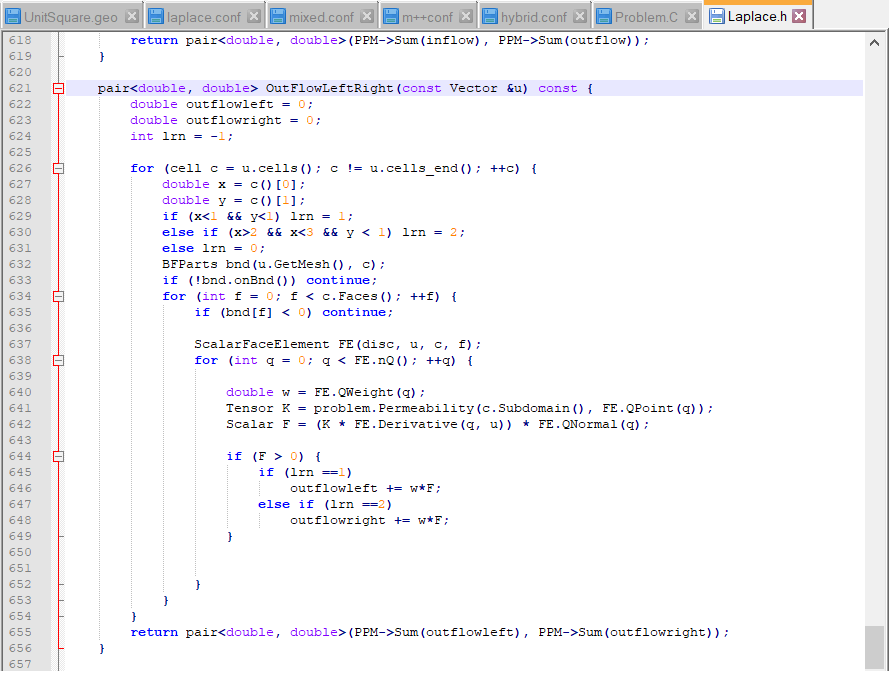
\includegraphics[width=\textwidth]{../../19/laplaceoutflow.png}
	
\end{figure}
Ähnlich wie zuvor bei den gemischten Finiten Elementen verfahren wir auch bei den linearen Finiten Elementen.
Es ändern sich lediglich die konkreten Berechnungen des Ausflusses. \newline
Somit ließen sich folgende Ergebnisse erzielen:
\begin{figure}[H]
	\centering
	\captionabove{Gitter und Permeabilität}
	\subfigure[hohe Permeabilität und grobes Gitter]{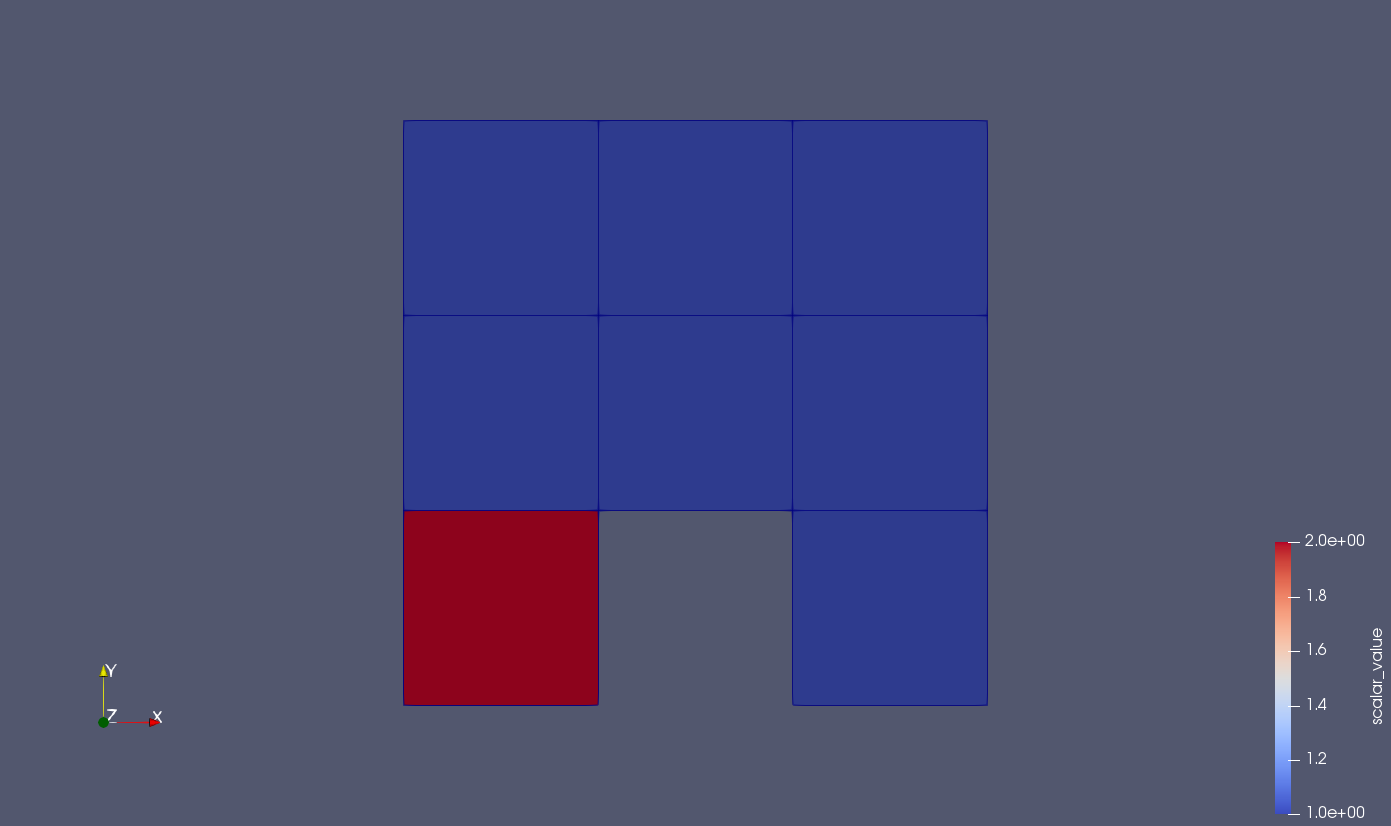
\includegraphics[width=0.49\textwidth]{../../19/perm20lvl0.png}}
	\subfigure[niedrige Permeabilität und feines Gitter]{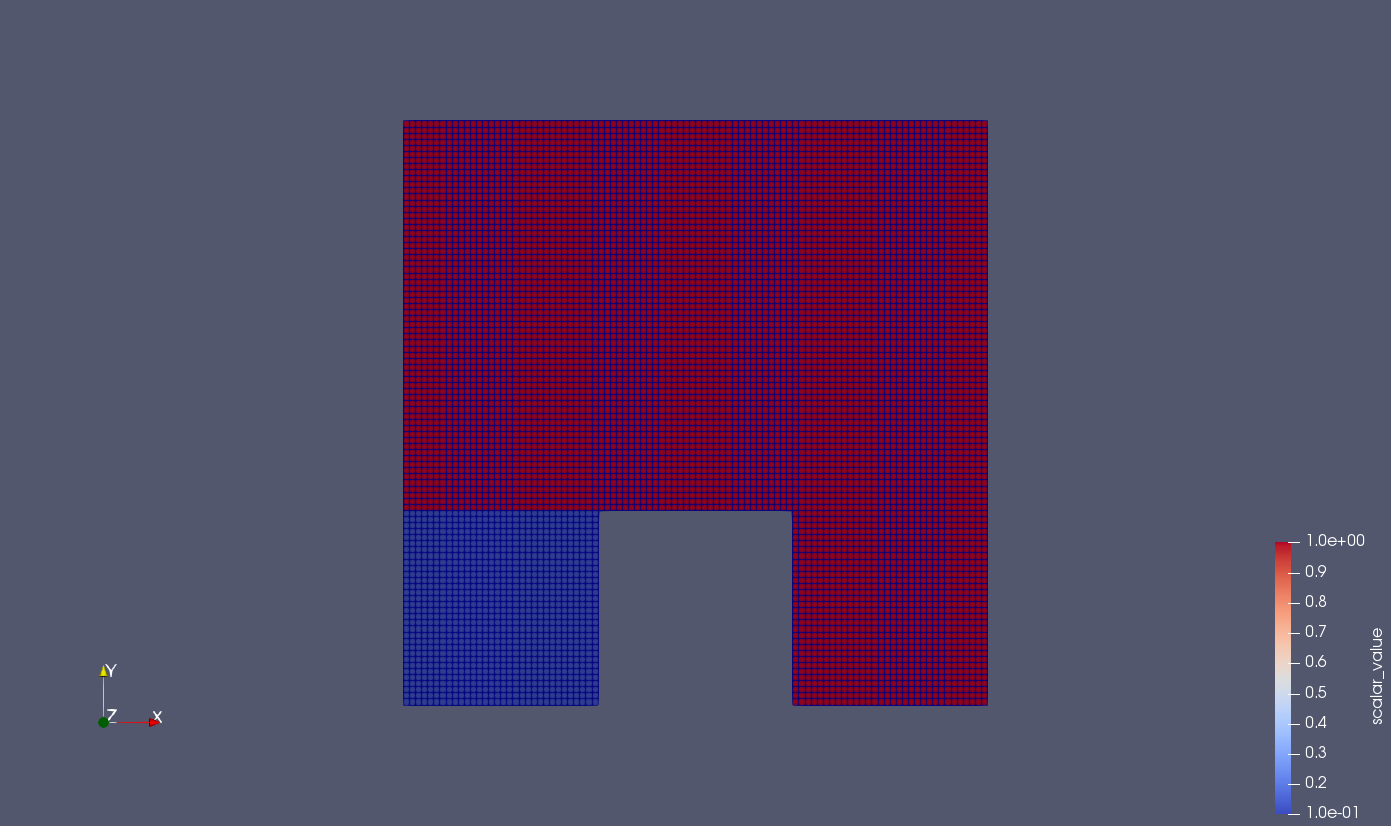
\includegraphics[width=0.49\textwidth]{../../19/perm01lvl5.png}}

\end{figure}

\begin{figure}[H]
	\centering
	\captionabove{Lösung mit niedriger Permeabilität auf hohem Level}
	
	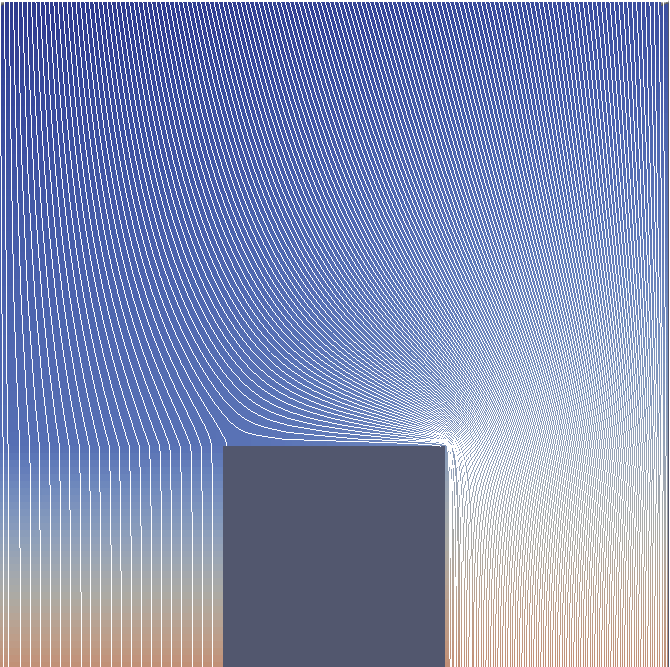
\includegraphics[width=\textwidth]{../../19/StreamLinesgemfem.png}
	
\end{figure}
Man kann sehr schön die an der rechten Ecke des Steins entstehende Singularität erkennen. Ebenso sieht man leicht, dass das Wasser auf seinem Weg nach unten das Gebiet mit niedrigerer Permeabilität meidet und eher rechts vom Stein versickert. 
Setzt man die Permeabilität der Lehmschicht hingegen höher,
ändert sich das Verhalten des Wassers dementsprechend:
\begin{figure}[H]
	\centering
	\captionabove{Lösung mit erhöhter Permeabilität auf hohem Level}
	
	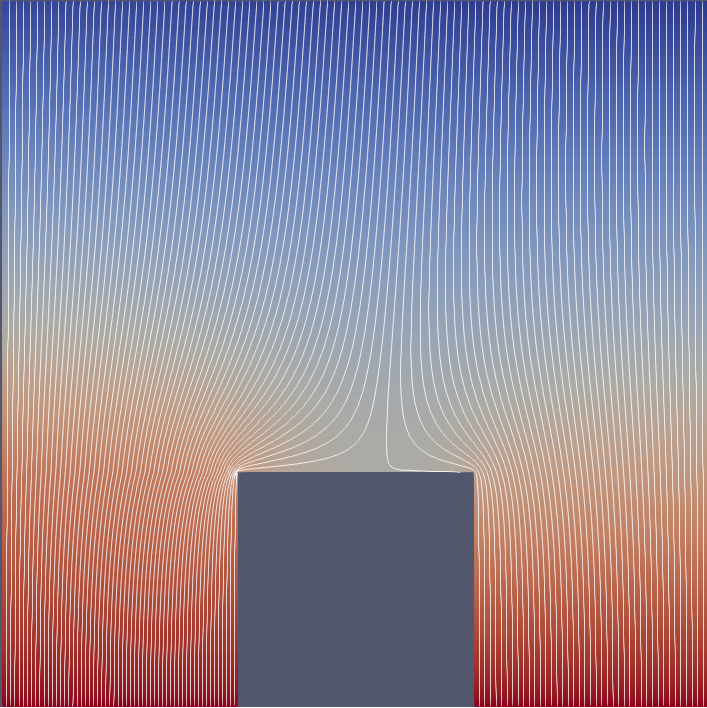
\includegraphics[width=\textwidth]{../../19/streamlines20lvl7.png}
	
\end{figure}

\newpage
\subsubsection{Daten und Interpretation}
\begin{figure}[H]
	\centering
	\captionabove{Aufgabe 18}
		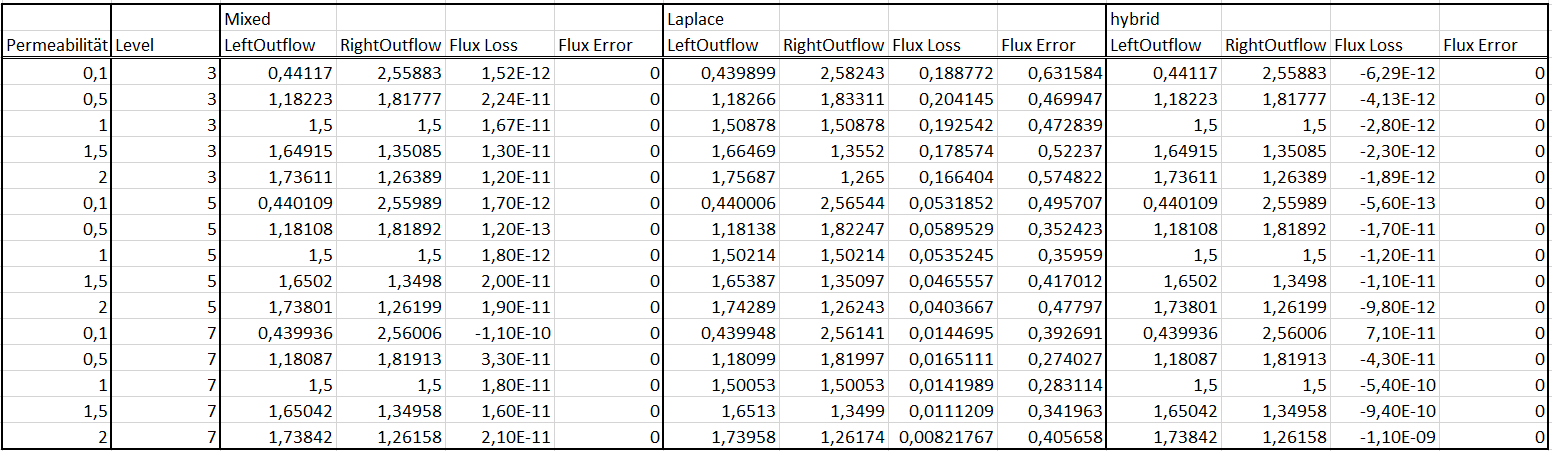
\includegraphics[width=\textwidth]{../../19/blatt5tabelle.png} 
\end{figure}
Wie schon bei den beiden vorherigen Tabellen bemerkt wurde, sieht man hier wieder schön, dass die gemischte und hybride Finite Elemente Methode die gleichen Ergebnisse bei LeftOutflow und RightOutflow liefern. \newline
Weiter sieht man bei diesen beiden Methoden, dass der Fluss erhalten wird, d.h. der Flux Loss ist extrem niedrig und im Bereich der zu erwartenden Ungenauigkeiten. \newline Im Gegensatz dazu erkennt man bei der linearen Finite Elemente Methode (Laplace), dass der Fluss nicht erhalten wird und auch deutlich schlechtere Ergebnisse insgesamt geliefert werden. \newline
Bei der Permeabilität 1 wird dieser Unterschied zwischen hybrid/mixed und linearen FEM am besten deutlich. Hierbei liefert die lineare Methode einen insgesamt zu hohen Ausfluss (z.B. bei Level 5 ist der Ausfluss 3,00428), wohingegen bei den anderen beiden der erwartete Wert von 1,5 auf beiden Seiten zustande kommt. 

\subsubsection{Extrapolation}

\begin{figure}[H]
	\centering
	\captionabove{Extrapolation mit gemischten FE}
	\subfigure[für 'leftoutflow' mit Permeabilität gegen 0]{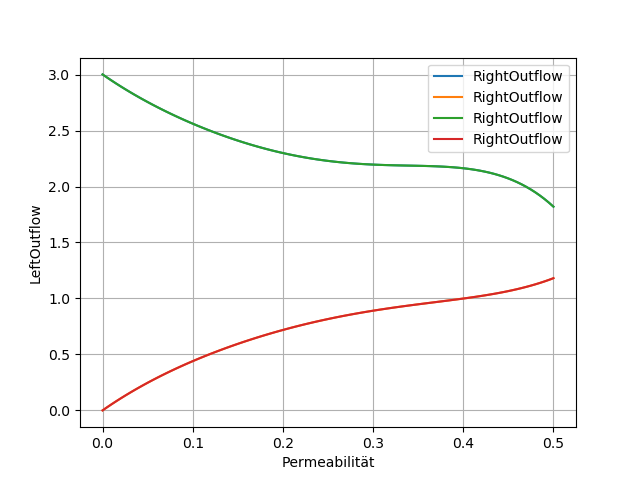
\includegraphics[width=0.49\textwidth]{../../19/mixlinks.png}}
	\subfigure[für 'rightoutflow' mit Permeabilität gegen 0]{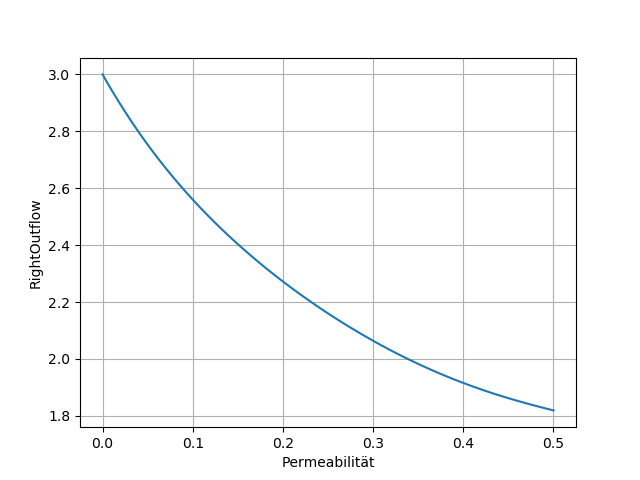
\includegraphics[width=0.49\textwidth]{../../19/mixrechts.png}}
	
\end{figure}

Es ergeben sich als Auswertung der Extrapolation mit Permeabilität gleich 0 die Werte: 
\begin{align*}
\text{'leftoutflow'} &= -3,82215 \cdot 10^{-6} \\
\text{'rightoutflow'} &= 2,9999953 
\end{align*}

\begin{figure}[H]
	\centering
	\captionabove{Extrapolation mit linearen FE}
	\subfigure[für 'leftoutflow' mit Permeabilität gegen 0]{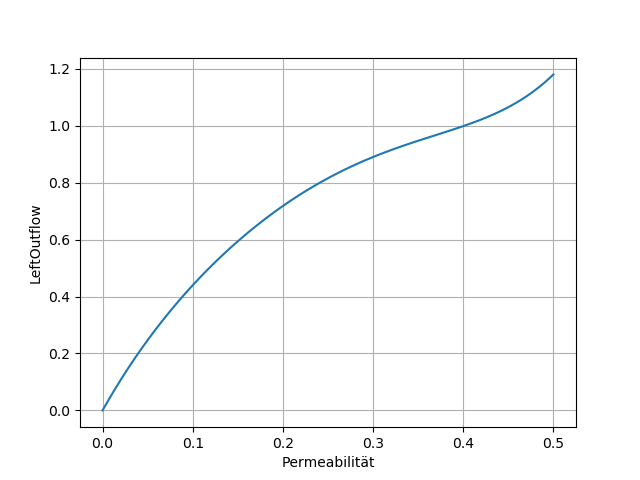
\includegraphics[width=0.49\textwidth]{../../19/linlinks.png}}
	\subfigure[für 'rightoutflow' mit Permeabilität gegen 0]{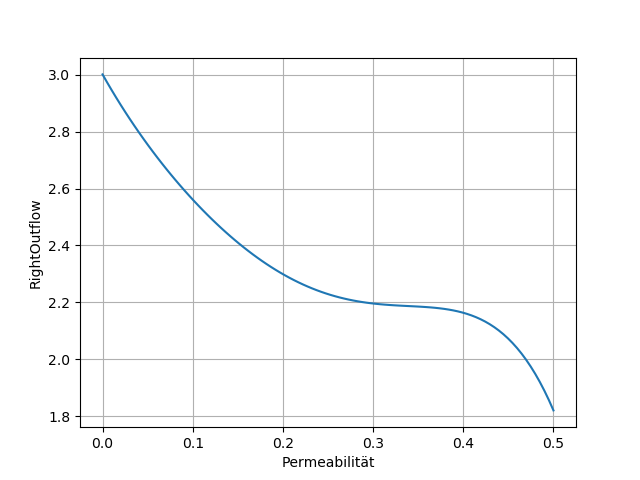
\includegraphics[width=0.49\textwidth]{../../19/linrechts.png}}
	
\end{figure}

Es ergeben sich als Auswertung der Extrapolation mit Permeabilität gleich 0 die Werte: 
\begin{align*}
\text{'leftoutflow'} &= 6.55787 \cdot 10^{-8} \\
\text{'rightoutflow'} &= 3.00159
\end{align*}




\begin{figure}[H]
	\centering
	\captionabove{Dabei sind wir wie folgt vorgegangen:}
	
	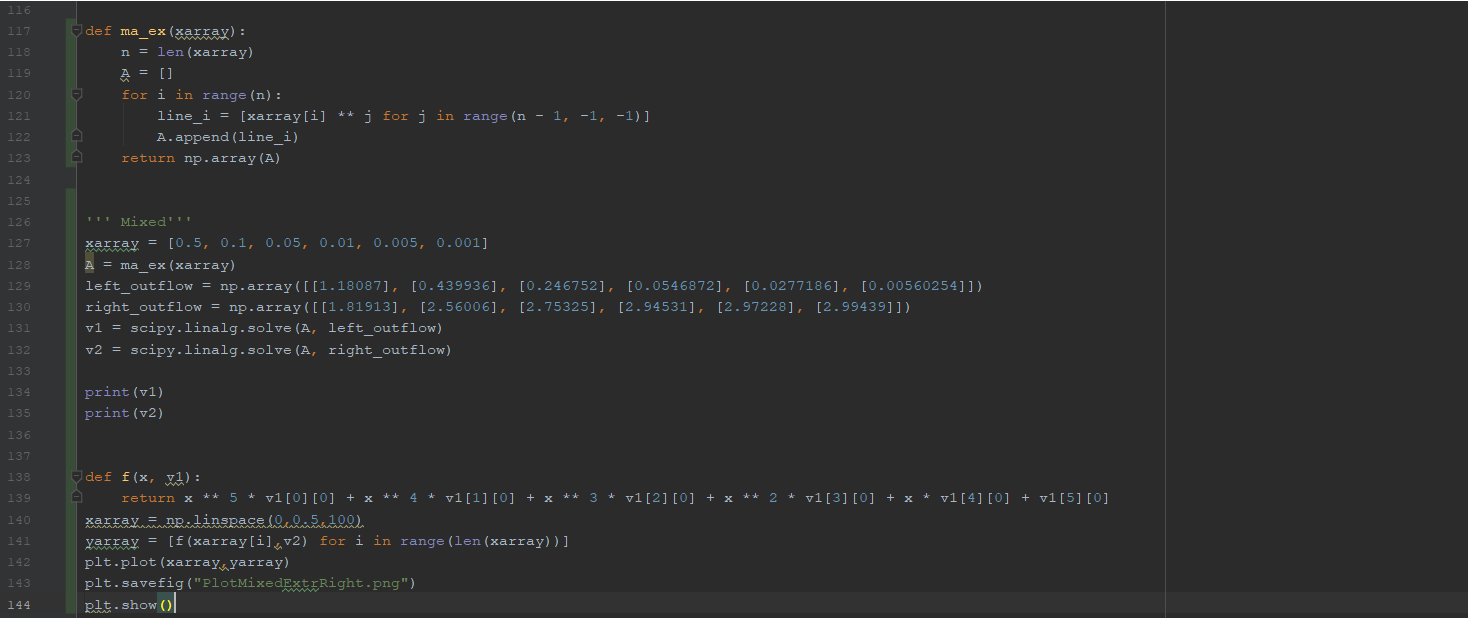
\includegraphics[width=\textwidth]{../../19/extrapolation.png}
	
\end{figure}